\subsubsection{Windows setup steps}
There are no special steps to follow for Windows; just click the `initial setup' button and watch the Python console for any errors. If everything worked, you should see a green success message.

\subsubsection{Mac OS setup steps}
\begin{enumerate}
    \item Click the `initial setup' button. It is likely this will fail and you may see an error similar to the image below. Select `\textbf{Cancel}'.
    \begin{figure}[h!]
        \centering
        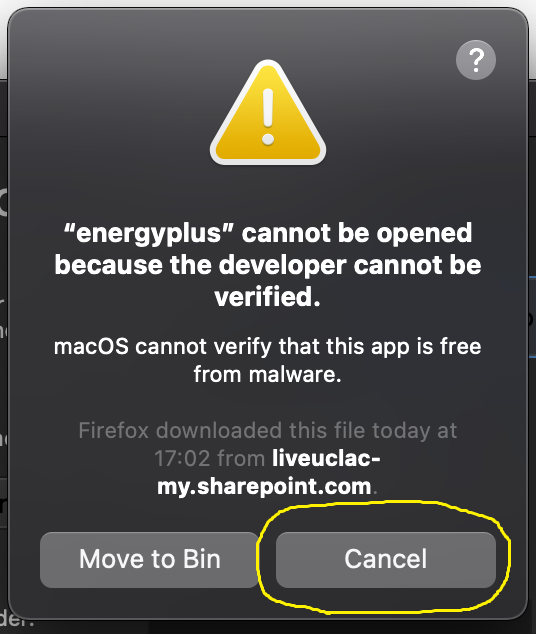
\includegraphics[width=5cm]{Screenshot 2022-06-22 at 20.30.52.png}
        %\caption{Click the initial setup button. It is likely this will fail and you may see an error similar to the image below. Select `\textbf{Cancel}'.}
        \label{fig:mac1}
    \end{figure}
    
    \item Navigate to \textbf{System Preferences $\rightarrow$ Security \& Privacy}.
    \clearpage
    
    \item You should now see a notice similar to the image below. Select `\textbf{Allow Anyway}'.
    \begin{figure}[h!]
        \centering
        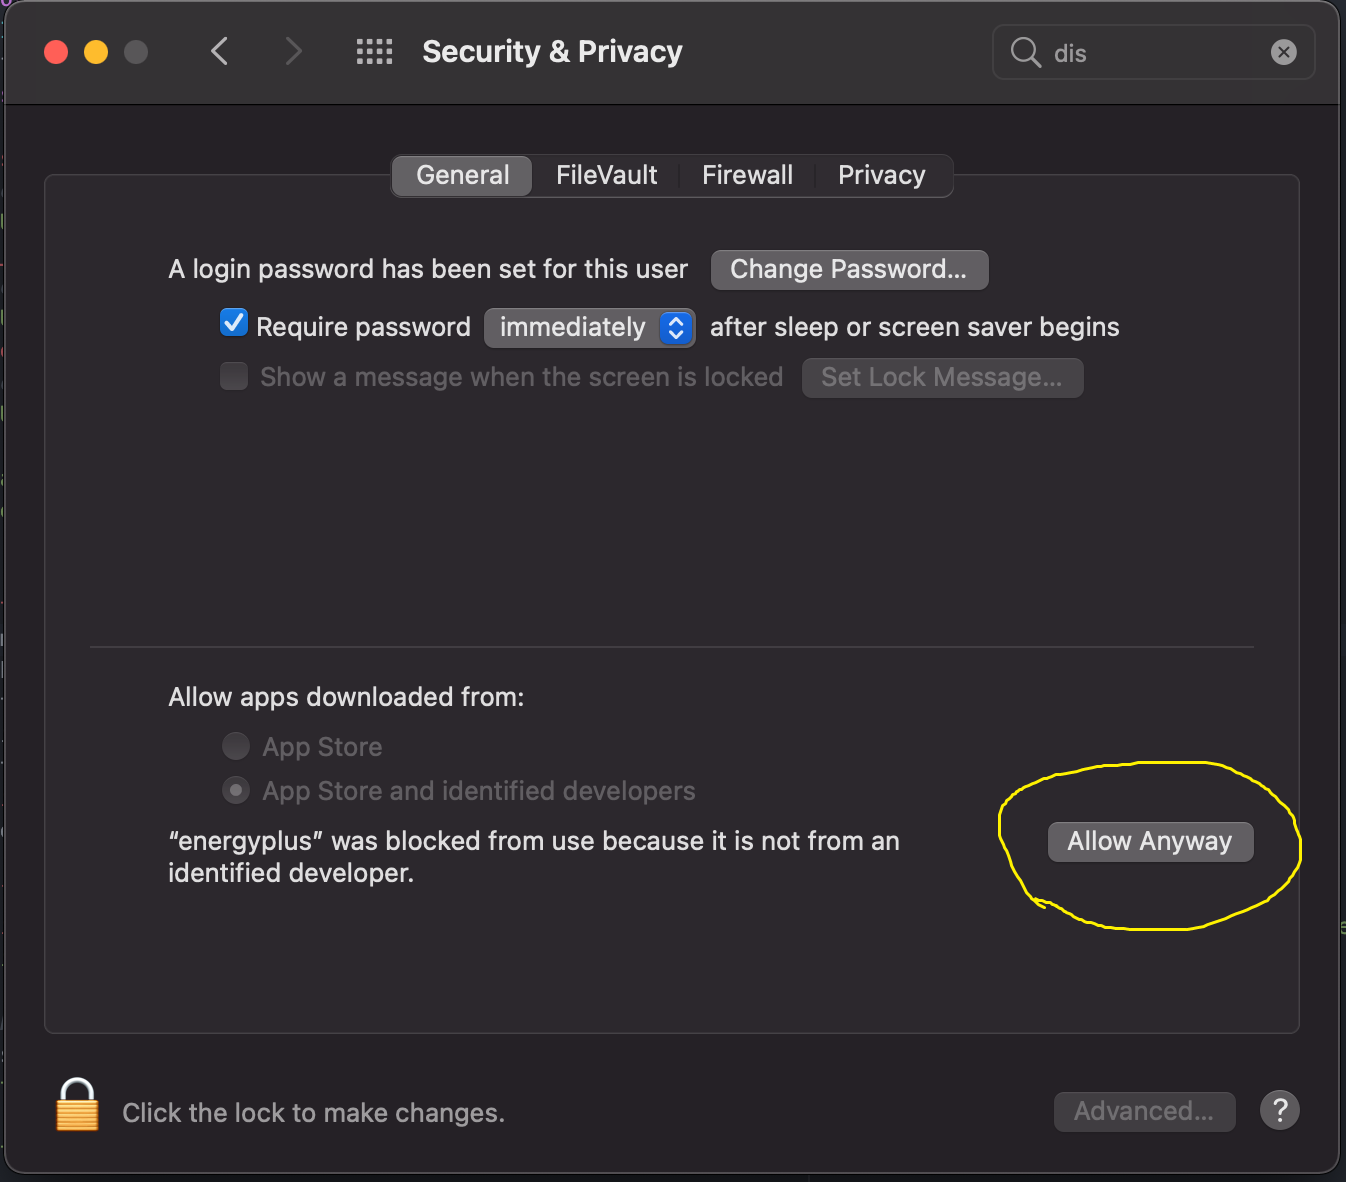
\includegraphics[width=10cm]{Screenshot 2022-06-22 at 20.31.15.png}
        \label{fig:mac2}
    \end{figure}
    
    \item Go back to the QGIS window and click the `initial setup' button again. A message similar to the image below will show up; select `\textbf{Open}'.
    \begin{figure}[h!]
        \centering
        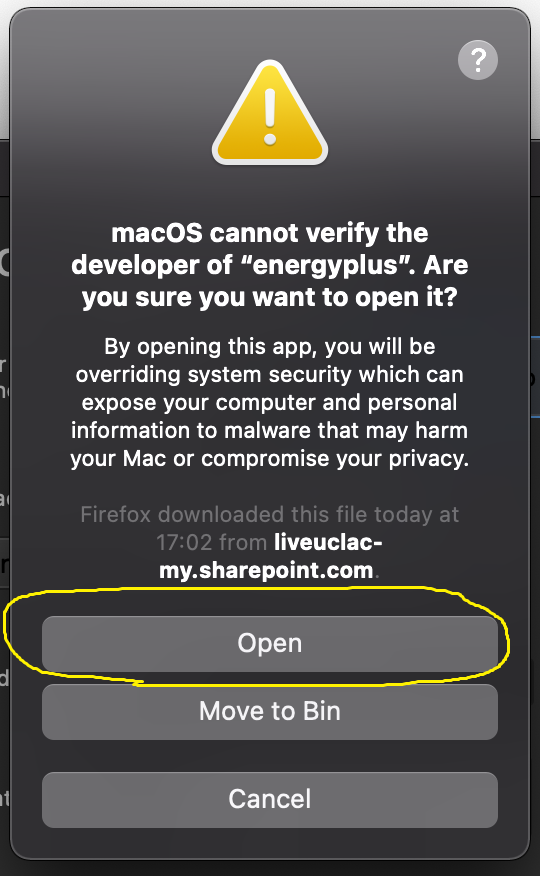
\includegraphics[width=5cm]{Screenshot 2022-06-22 at 20.32.14.png}
        \label{fig:mac3}
    \end{figure}
    \clearpage
    
    \item You should now see another error (below), almost identical to the message in step~1. If you don't see this, try clicking the `initial setup' button again. If this still does not appear, restart QGIS and click the `initial setup' button. Once you see the error below, select `\textbf{Cancel}'.
    \begin{figure}[h!]
        \centering
        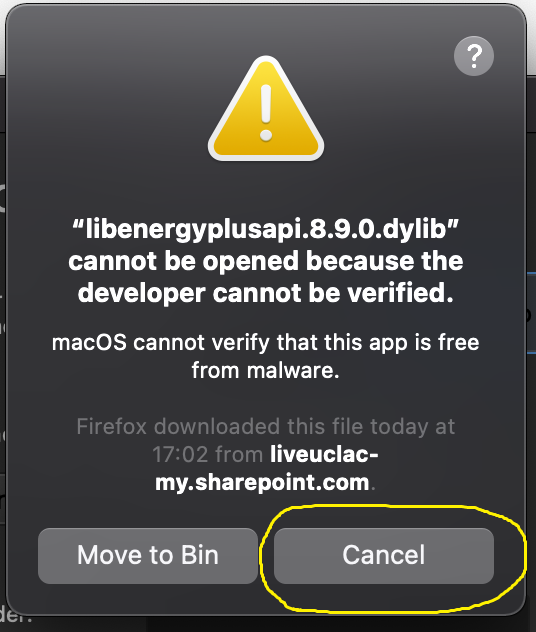
\includegraphics[width=5cm]{Screenshot 2022-06-22 at 20.32.27.png}
        \label{fig:mac4}
    \end{figure}
    
    \item Again, navigate to \textbf{System Preferences $\rightarrow$ Security \& Privacy}.
    
    \item Select `\textbf{Allow Anyway}'.
    \begin{figure}[h!]
        \centering
        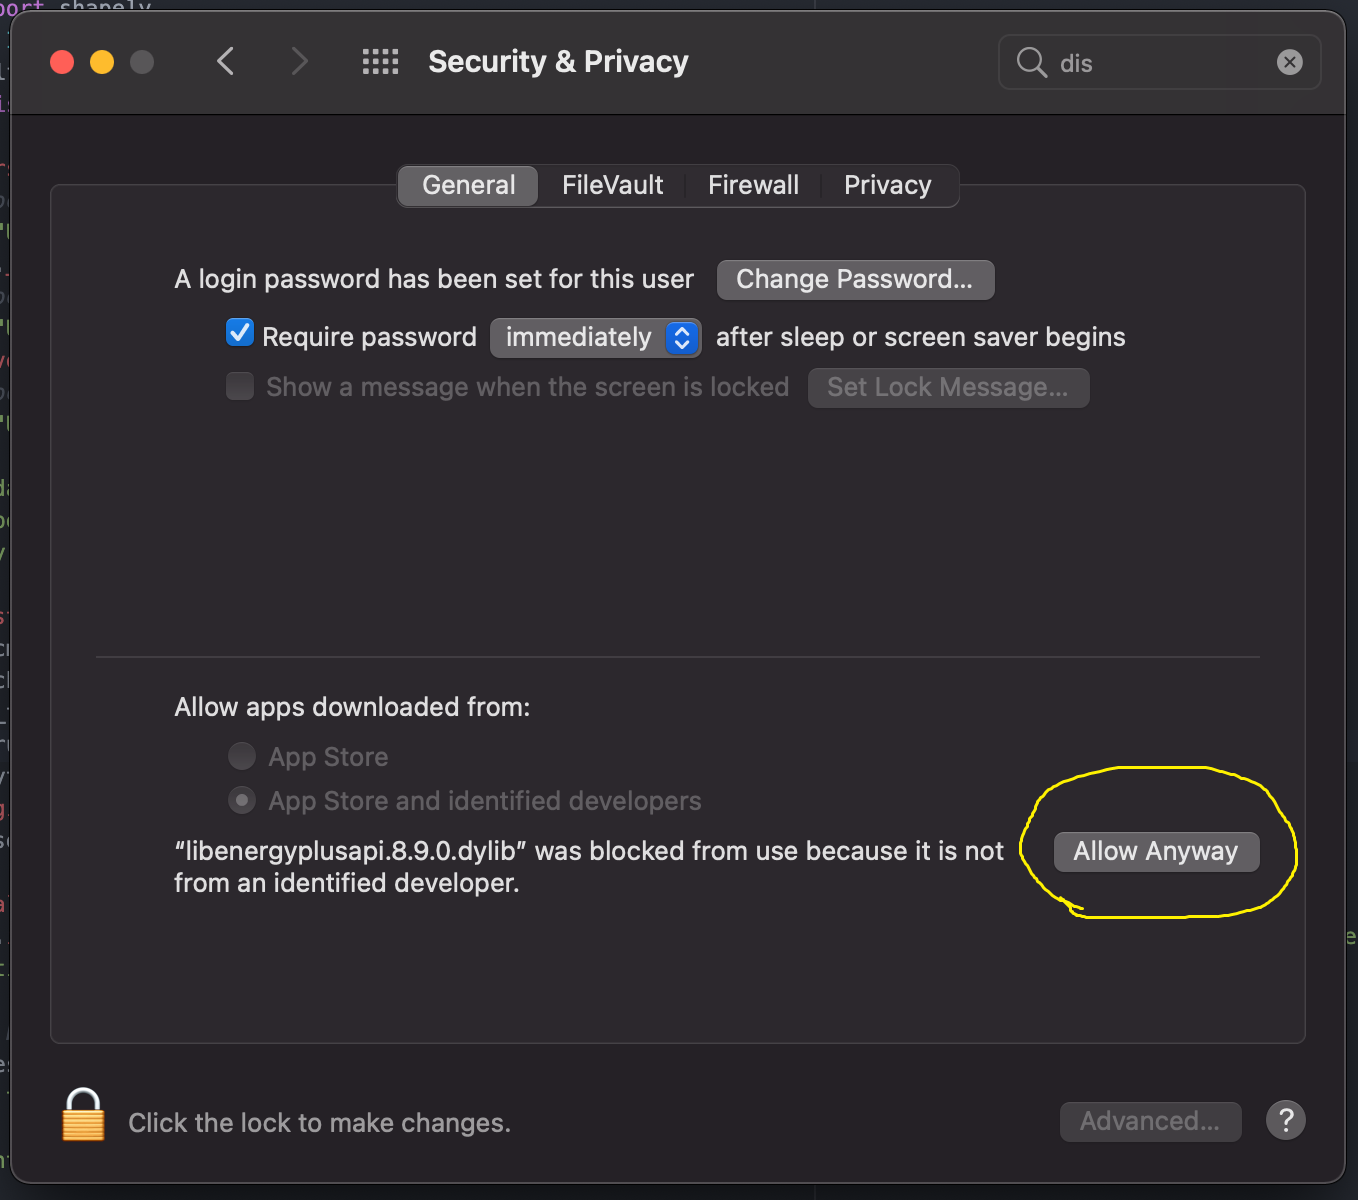
\includegraphics[width=10cm]{Screenshot 2022-06-22 at 20.32.54.png}
        \label{fig:mac5}
    \end{figure}
    \clearpage
    
    \item Finally, click the `initial setup' button again back in QGIS. You should see the dialogue below; select `\textbf{Open}'.
    \begin{figure}[h!]
        \centering
        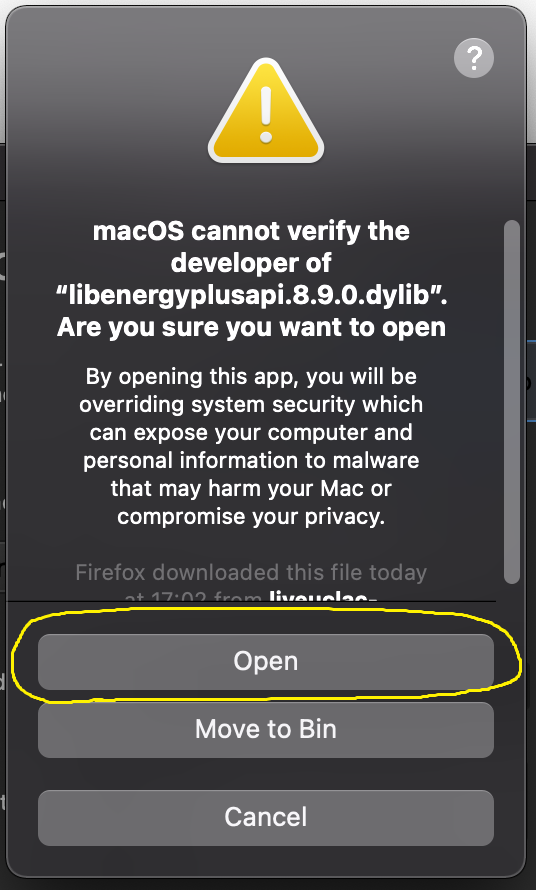
\includegraphics[width=5cm]{Screenshot 2022-06-22 at 20.33.15.png}
        \label{fig:mac6}
    \end{figure}
    
    \item The plugin should now be fully functioning - though you may need to restart QGIS for a final time. You can check if the setup has worked by clicking the `initial setup' button; if everything is functioning correctly, there should be a green confirmation message in QGIS.
    
\end{enumerate}